
In this section, well known standards will be investigated.

\begin{itemize}
    \item American Society of Mechanical Engineers (ASME):
	    \begin{itemize}[label=$\bullet$]
	    	\item Boiler and Pressure Vessel Code, Section VII, Division 1, 2015 \citep{ASMEbvpcVII1}
	    	\item Boiler and Pressure Vessel Code, Section VII, Division 2, 2015 \citep{ASMEbvpcVII2}
%	    	\item Boiler and Pressure Vessels for Human Occupancy
	    \end{itemize}
	\item Det Norske Veritas(DNV) \citep{DNVOSD101}
		    \begin{itemize}[label=$\bullet$]
	    	\item DNV-OS-D101, Marine and Machinery Systems and Equipment\citep{ASMEbvpcVII1}
	    \end{itemize}
    \item European Standard EN
        \begin{itemize}[label=$\bullet$]
	       	\item EN 13445-3:2014
	    \end{itemize}
\end{itemize}

\section{ASME BPVC}

\subsection{Section VII: Division 1}
As per UG-28 of \citep{ASMEbvpcVII1}, the following procedure was used to calculate the required thickness.\\

The following list of steps were carried out as per \citep{ASMEbvpcVII1}\\

\begin{enumerate}
	\item Assume initial thickness value of $t$
	\item Calculate $D_o/t$ ratio and assure $D_o/t \geq 10$.
	\item Calculate $L/D_o$ ratio, if $L/D_o \geq 50 \Rightarrow 50$ or  $L/D_o \leq 0.05 \Rightarrow 0.05$
	\item With above ratios, go to Figure G of \citep{ASMEbvpcIID} and get value for $A$
	\item With $A$ from above go to chart CS-2 $\because S_y \geq 30 \ ksi$ to get $B$
	\item Using $B$ use Equation \ref{eq:3_VII_1_stp6} to calculate allowable pressure $p_a$:
		\begin{equation}
			\label{eq:3_VII1_stp6}
			p_a = \frac{4B}{3 \left(\frac{D_o}{t} \right)}
		\end{equation}
	\item Check if $p_a \geq p_{req}$ as calculated from \ref{eq:2_preq}, if not, incease $t$ and go to Step 1
	
\end{enumerate}

With the Python Script in REFAPPENDIX the convergence plot from Figure~\ref{fig:3_vii1_cnvg} below was created.
\begin{figure}[!htbp]
    \centering
    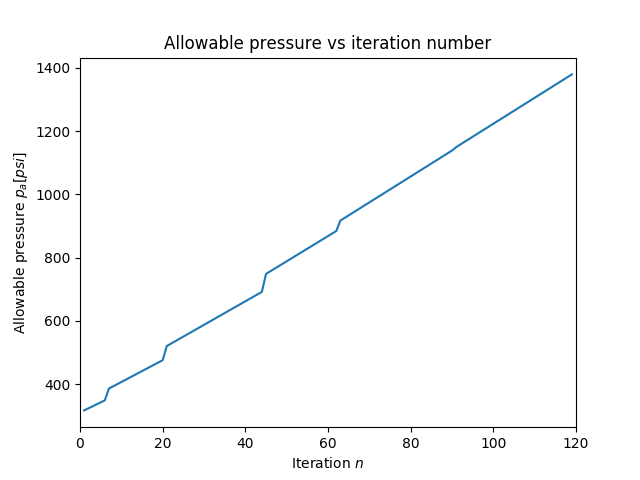
\includegraphics[]{3_vii1_cnvg}
    \caption{Convergence plot of $p_a$.}
    \label{fig:3_vii1_cnvg}
\end{figure}

The script converged at thickness of $t = 1.68\ in$ and an allowable pressure of $p_a = 1379.4\ psi$ after 119 iterations. 


\subsection{Section VII: Division 2}
As per subsection 4.4.5 of \citep{ASMEbvpcVII2}, the following procedure was used to calculate the required thickness. Note that only the main formulas will be presented. For intermediate steps, see REFAPPENDIX X for Python script utilized during iteration.\\

The following list of steps were carried out as per \citep{ASMEbvpcVII2}\\

\begin{enumerate}
	\item Assume initial thickness value of $t$
	\item Calculate elastic buckling stress $F_{he}$ with \ref{eq:3_VII2_4419}
		\begin{equation}
			\label{eq:3_VII2_4419}
			F_{he} = \frac{1.6\ C_h E_y t}{D_o}
		\end{equation}
	\item Based on $S_y$ and $F_{he}$, calculate the predicted buckling stress $F_{ic}$
	\item With subsection 4.4.2 of \citep{ASMEbvpcVII2}, compute the design factor $FS$
	\item Calculate allowable pressure $p_a$ with \ref{eq:3_VII2_4428}
		\begin{equation}
			\label{eq:3_VII2_4428}
			p_a = 2 F_{ha} \left(\frac{t}{D_o}\right)
		\end{equation}
	\item Check if $p_a \geq p_{req}$ as calculated from \ref{eq:2_preq}, if not, increase $t$ and go to Step 1
	
\end{enumerate}

With the Python Script in REFAPPENDIX the convergence plot from Figure~\ref{fig:3_vii2_cnvg} below was created.
\begin{figure}[!htbp]
    \centering
    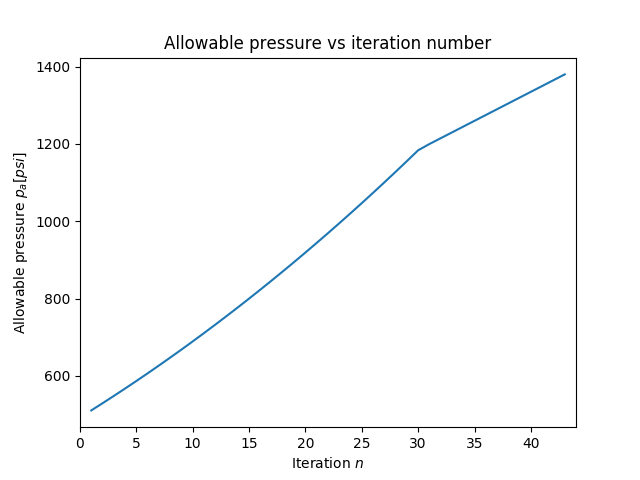
\includegraphics[]{3_vii2_cnvg}
    \caption{Convergence plot of $p_a$.}
    \label{fig:3_vii2_cnvg}
\end{figure}

The script converged at thickness of $t = 0.92\ in$ and an allowable pressure of $p_a = 1379.7\ psi$ after 43 iterations. 

\section{DNV}

\subsection{DNV-OS-D101}

As per \citep{DNVOSD101}, in subsection F215, Equation~\ref{eq:3_DNV_hoop} is presented as follows.

\begin{equation}
	\label{eq:3_DNV_hoop}
	\sigma_h = C\cdot\frac{T}{d_{thr}t}
\end{equation}

In this equation, $C$ is a factor based on the number of wraps on the drum,. for two layers $C=1.75$. It is also to be noted that the hoop stress is limited to $\sigma_h \leq 0.85\cdot S_y$. \\

For this application, rearranging for $t$, setting $\sigma_h = S_{allow}$ and solving accordingly will yield a valid value of $t = 1.44 \ in$. 

\section{European European Standard EN}

\section{Comparison}

